\normaltrue \difficilefalse \tdifficilefalse
\correctionfalse

%\UPSTIidClasse{11} % 11 sup, 12 spé
%\newcommand{\UPSTIidClasse}{12}

\subsection*{Lokomat $\star$ \label{C2:06:93}}
\marginnote{\textit{CCINPT -- TSI -- 2023.}}
\marginnote{\UPSTIcompetence[2]{C2-06}}
\marginnote{\UPSTIcompetence[2]{A3-05}}
\setcounter{question}{0}

\index{Compétence C2-06}
\index{Lokomat}

%\index{Train d'engrenages simple}
\ifcorrection
\else
\marginnote{\textbf{Pas de corrigé pour cet exercice.}}
\fi

\ifprof
\else


Le réducteur utilisé est un réducteur de type train épicycloïdal à trois étages. Un schéma 
cinématique est fourni ci-dessous. 
On note $D_i$ le diamètre de la roue dentée $i$ , $i\in \lbracket 0,3 \rbracket$. 


\begin{center}
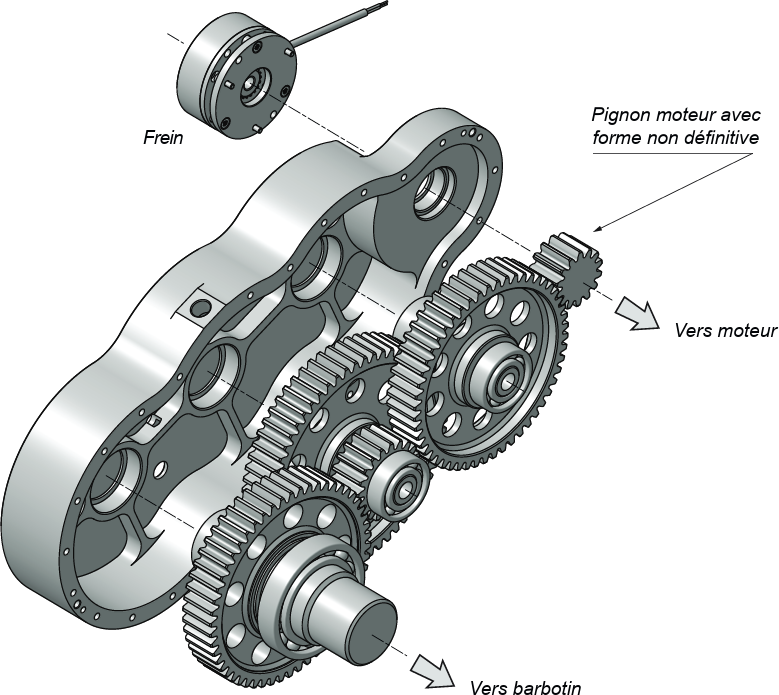
\includegraphics[width=\linewidth]{92_01}
\end{center}

On donne le nombre de dents $Z_i$ des éléments constitutifs $i$ du premier étage du train épicycloïdal : 
 $Z_0 = \SI{60}{dents}$,  $Z_1 = \SI{18}{dents}$,  $Z_2 = \SI{45}{dents}$,  $Z_3 = \SI{24}{dents}$.
 
\fi


\question{Calculer le rapport de transmission du premier étage.}
\ifprof
\else
\fi

\question{Les étages étant tous identiques, en déduire le rapport de transmission global du réducteur.}
\ifprof ~\\

\else
\fi

 

\ifprof
\else
\begin{flushright}
\footnotesize{Corrigé  voir \ref{C2:06:93}.}
\end{flushright}%
\fi